\documentclass[12pt, letterpaper]{article}

% --- Packages ----------------------------------------------------------------
\usepackage[utf8]{inputenc}
\usepackage[T1]{fontenc}
\usepackage[margin=1in]{geometry}
\usepackage{graphicx}
\usepackage{titlesec}
\usepackage{fancyhdr}
\usepackage{booktabs}
\usepackage{array}
\usepackage{tabularx}
\usepackage{float}
\usepackage{caption}
\usepackage{amsmath}
\usepackage{enumitem}
\usepackage{xcolor}
\usepackage{listings}
\usepackage{parskip}
\usepackage{hyperref}

% --- Colors ------------------------------------------------------------------
\definecolor{cppgreen}{RGB}{0,100,60}
\definecolor{cppdarkgreen}{RGB}{0,75,35}
\definecolor{cppgold}{RGB}{198,166,84}

% --- Header / Footer ---------------------------------------------------------
\pagestyle{fancy}
\fancyhf{}
\renewcommand{\headrulewidth}{0.4pt}
\lhead{Cal Poly Pomona -- Autonomous Vehicle Laboratory -- IGVC 2026 AutoNav}
\rfoot{\thepage}

% --- Section formatting ------------------------------------------------------
\titleformat{\section}{\Large\bfseries}{}{0em}{\thesection.~}
\titleformat{\subsection}{\large\bfseries}{}{0em}{\thesubsection~}

% --- Hyperref setup ----------------------------------------------------------
\hypersetup{
    colorlinks=true,
    linkcolor=cppdarkgreen,
    urlcolor=cppdarkgreen,
    citecolor=cppdarkgreen
}

% --- Code listing style ------------------------------------------------------
\lstset{
    basicstyle=\ttfamily\small,
    keywordstyle=\color{cppdarkgreen}\bfseries,
    commentstyle=\color{gray},
    stringstyle=\color{cppgold},
    breaklines=true,
    frame=single,
    numbers=left,
    numberstyle=\tiny\color{gray},
    tabsize=4
}

% =============================================================================
\begin{document}

% --- Title Page --------------------------------------------------------------
\begin{titlepage}
\centering

\vspace*{1cm}

% Replace with actual logo files:
% \includegraphics[height=1.5cm]{figures/avl_logo.png}
% \hfill
% \includegraphics[height=1.5cm]{figures/cpp_logo.png}

{\Large\textbf{California State Polytechnic University, Pomona}}\\[0.3cm]
{\LARGE\textbf{Autonomous Vehicle Laboratory}}\\[0.3cm]
{\Large\textbf{IGVC 2026 Design Report}}\\[1.2cm]

{\fontsize{36}{42}\selectfont\textbf{\textit{ROBOT NAME}}}\\[1.5cm]

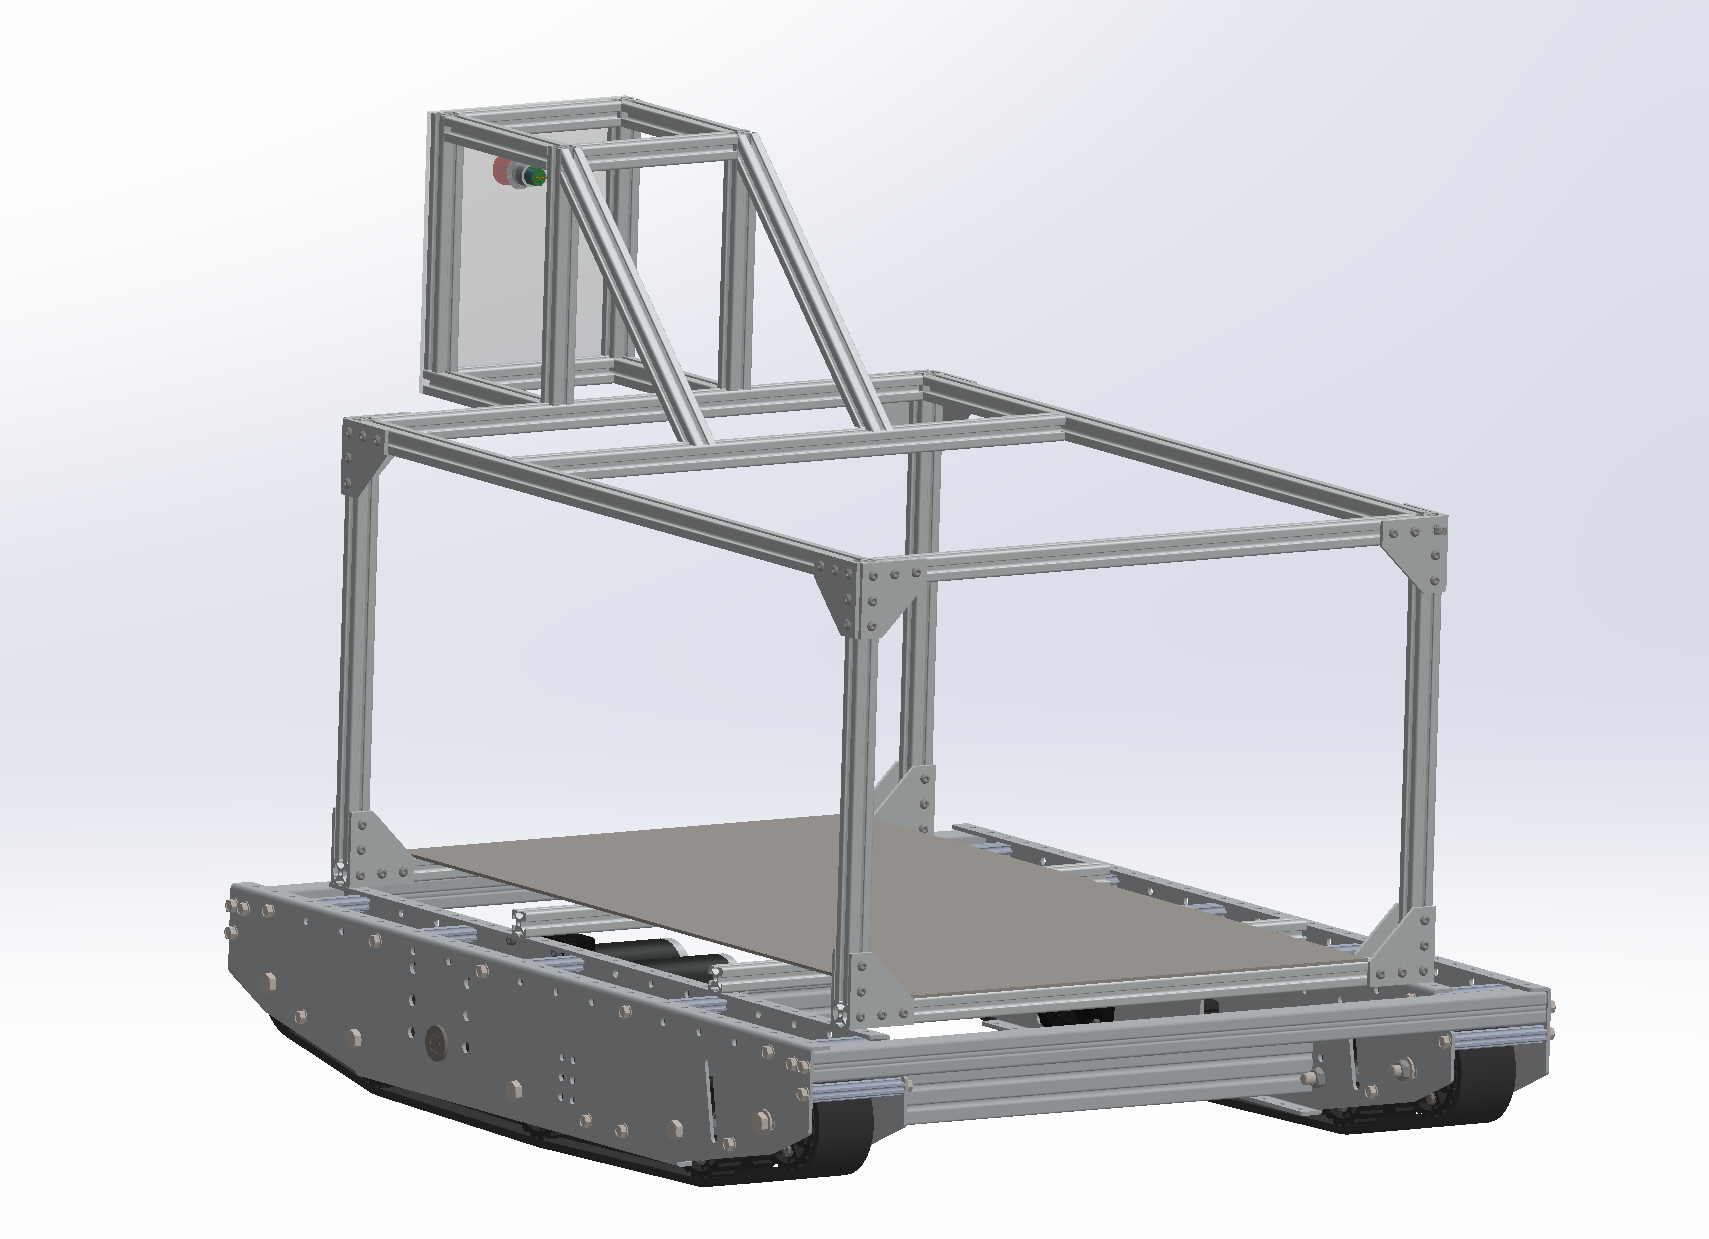
\includegraphics[width=0.55\textwidth]{figures/mech_image1.png}

\vspace{2cm}

\begin{minipage}{0.8\textwidth}
\centering
I hereby certify that the development of the vehicle, \textit{ROBOT NAME}, as described in this report, is equivalent to the work involved in a senior design course.\\[1.5cm]

\rule{8cm}{0.4pt}\\
Submitted May XX, 2026
\end{minipage}

\vspace{1.5cm}

\begin{tabular}{ccc}
\textbf{Software} & \textbf{Mechanical} & \textbf{Electrical} \\
\midrule
Name & Name (Captain) & Name \\
Name & Name & Name \\
Name & Name & Name \\
Name &  &  \\
\end{tabular}

\end{titlepage}

% --- Table of Contents -------------------------------------------------------
\thispagestyle{fancy}
\tableofcontents
\newpage

% =============================================================================
% SECTION 1
% =============================================================================
\section{Design Process, Team Identification and Organization}

\subsection{Introduction}

The Autonomous Vehicle Laboratory (AVL), representing California State Polytechnic University, Pomona (Cal Poly Pomona) and the College of Engineering, proudly presents \textit{ROBOT NAME}, our entry for the 2026 Intelligent Ground Vehicle Competition (IGVC) in the AutoNav category. AVL is a multidisciplinary student organization within the College of Engineering, with a dedicated IGVC team of XX students. The team is advised by ADVISOR NAME(S), faculty member(s) at Cal Poly Pomona.

Cal Poly Pomona's learn-by-doing philosophy is at the core of AVL's approach. Every component of the vehicle---from mechanical design to embedded firmware to autonomous navigation software---is designed, built, and tested by students. This is the team's first entry in the IGVC competition.

\subsection{Team Organization}

The IGVC team is organized into three specialized subteams: electrical, mechanical, and software. A team captain serves as the primary point of contact with AVL leadership and faculty advisors, providing regular updates on progress and coordinating across subteams.

\begin{itemize}[nosep]
    \item \textbf{Mechanical:} Chassis design, drivetrain, sensor mounting, weatherproofing
    \item \textbf{Electrical:} Power distribution, motor controllers, PCB design, CAN bus, e-stop
    \item \textbf{Software:} Perception, navigation, localization, firmware, GUI
\end{itemize}

To promote communication and prevent silos, the team holds weekly full-team meetings in addition to subteam work sessions. All design decisions are documented and version-controlled.

\subsection{Design Process}

To develop \textit{ROBOT NAME}, the team implemented an iterative design process that focuses on a cycle of researching, designing, prototyping, and testing.

% \begin{figure}[H]
%     \centering
%     \includegraphics[width=0.7\textwidth]{figures/design_process.png}
%     \caption{Iterative design process.}
%     \label{fig:design_process}
% \end{figure}

\begin{enumerate}[nosep]
    \item \textbf{Define} --- Establish system-level requirements from competition rules.
    \item \textbf{Research} --- Survey existing solutions, reference designs, and prior IGVC reports.
    \item \textbf{Design} --- Create detailed CAD models, schematics, and software architecture.
    \item \textbf{Prototype} --- Build rapid prototypes (3D-printed parts, breadboard circuits, simulation).
    \item \textbf{Test} --- Validate each subsystem independently, then integrate.
    \item \textbf{Implement} --- Finalize manufacturing and deploy to the competition vehicle.
\end{enumerate}

The team began by analyzing design reports from prior IGVC winners and performing a full re-read of the 2026 competition rules to derive a list of rule-based requirements. From these, the team established high-level design goals. With the system-level requirements defined, subteams proceeded to research, design, build, and test the necessary components. As each subsystem was completed, integration testing ensured that all components worked cohesively and that the robot met its overall requirements.

\newpage

% =============================================================================
% SECTION 2
% =============================================================================
\section{System Architecture}

\subsection{Mechanical and Electrical Architecture}

At a high level, \textit{ROBOT NAME} consists of several independent subsystems: chassis and tracked drivetrain, vision, sensors, and electronics.

\begin{figure}[H]
    \centering
    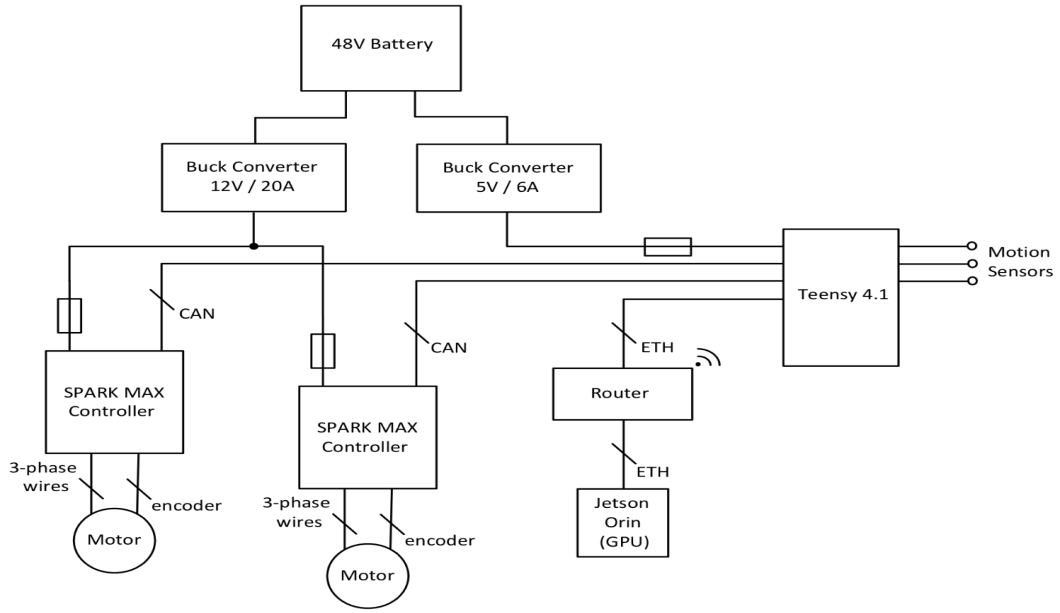
\includegraphics[width=0.85\textwidth]{figures/electrical_p1_img1.png}
    \caption{High-level electronic and power system architecture.}
    \label{fig:sys_arch}
\end{figure}

\begin{table}[H]
\centering
\caption{Major subsystems overview.}
\begin{tabularx}{\textwidth}{lX}
\toprule
\textbf{Subsystem} & \textbf{Description} \\
\midrule
Chassis          & AndyMark Raptor Track Drive with 80/20 T-slot aluminum extrusion frame and 1/8\,in diamond plate steel base (21.5\,in $\times$ 30\,in) \\
Drivetrain       & Tracked differential drive (skid-steer) with 2$\times$ REV SparkMAX controllers and NEO brushless motors \\
Compute          & NVIDIA Jetson Orin (GPU) for vision processing and object detection \\
Microcontroller  & Teensy 4.1 --- CAN bridge between main computer and motor controllers \\
Sensors          & TODO: Camera(s), GPS/IMU, motion sensors \\
Power            & 48\,V battery with dual buck converters (12\,V/20\,A for motors, 5\,V/6\,A for Teensy 4.1) \\
\bottomrule
\end{tabularx}
\end{table}

\subsection{Robot Safety}

\textit{ROBOT NAME} was designed with safety as a fundamental principle. Power is delivered to the drive motors only when the following conditions are simultaneously met:

\begin{enumerate}[nosep]
    \item The \textbf{remote emergency stop} is inactive (wireless e-stop not triggered).
    \item The \textbf{physical emergency stop} button on the vehicle is not pressed.
    \item The \textbf{software emergency stop} has not been asserted.
\end{enumerate}

If any one of these is triggered, motor power is immediately cut. To prevent accidental re-engagement, each of the three signals is also monitored redundantly in software. As a result, the robot will not send any non-zero command to the motors unless all safety interlocks are satisfied.

\subsection{Software Architecture}

The software is split into four major subsystems: sensors, perception, localization, and navigation.

% \begin{figure}[H]
%     \centering
%     \includegraphics[width=0.9\textwidth]{figures/software_architecture.png}
%     \caption{Software architecture and data flow.}
%     \label{fig:sw_arch}
% \end{figure}

\begin{itemize}[nosep]
    \item \textbf{Sensors} --- Camera capture, GPS/IMU reading, motor encoder feedback
    \item \textbf{Perception} --- GPU-accelerated image processing, obstacle detection, lane detection (Jetson Orin)
    \item \textbf{Localization} --- Sensor fusion (track odometry + GPS) for position estimation
    \item \textbf{Navigation} --- Path planning and motor command generation
\end{itemize}

Organizing the code in this modular way allows for easy testing of each subsystem independently as well as making testing different algorithms or parameters quick and easy.

\subsection{Robot Communication Bus}

Data is communicated between devices using the \textbf{CAN bus} protocol, a robust standard widely used in the automotive industry. The Teensy 4.1 microcontroller serves as the CAN bridge between the main onboard computer and the REV SparkMAX motor controllers.

The CAN bus operates at \textbf{1\,Mbit/s} using 29-bit extended frames. A CAN transceiver (SN65HVD230) converts the Teensy's logic-level signals to differential CAN\_H / CAN\_L. The bus is terminated with 120\,$\Omega$ resistors at each end.

% \begin{figure}[H]
%     \centering
%     \includegraphics[width=0.8\textwidth]{figures/can_bus_diagram.png}
%     \caption{CAN bus topology.}
%     \label{fig:can_bus}
% \end{figure}

\subsection{Bill of Materials}

The total cost to construct \textit{ROBOT NAME} was approximately \$X,XXX.

\begin{table}[H]
\centering
\caption{Major COTS components.}
\begin{tabularx}{\textwidth}{Xccr}
\toprule
\textbf{Major COTS Item} & \textbf{Qty} & \textbf{Market Cost (USD)} & \textbf{Team Cost (USD)} \\
\midrule
NVIDIA Jetson Orin               & 1 & \$TODO & \$TODO \\
TODO: Camera(s)                 & TODO & \$TODO & \$TODO \\
48\,V Battery                   & 1 & \$TODO  & \$TODO \\
TODO: GPS/IMU                   & 1 & \$TODO & \$TODO \\
AndyMark Raptor Track Drive     & 1 & \$TODO & \$TODO \\
REV SparkMAX + NEO Motor        & 2 & \$TODO & \$TODO \\
Teensy 4.1                      & 1 & \$30.00  & \$30.00 \\
CAN Transceiver (SN65HVD230)    & 1 & \$5.00   & \$5.00 \\
Buck Converters (12\,V + 5\,V)  & 2 & \$TODO   & \$TODO \\
Router                          & 1 & \$TODO   & \$TODO \\
\bottomrule
\end{tabularx}
\end{table}

\newpage

% =============================================================================
% SECTION 3
% =============================================================================
\section{Effective Innovations}

\subsection{Innovation 1: Cost-Effective Tracked Platform with Modular Frame}

As first-year participants, the team made the strategic decision to build on a commercially available AndyMark Raptor Track Drive platform combined with 80/20 T-slot aluminum extrusions. This approach provides several advantages over a fully custom chassis:

\begin{itemize}[nosep]
    \item \textbf{Reduced development time} --- By using a proven tracked drive platform, the team could focus development effort on sensors, electronics, and software rather than chassis fabrication.
    \item \textbf{Superior traction} --- The tank-track configuration spreads the vehicle's weight over a larger contact area compared to wheels, providing better traction and stability on uneven terrain and the competition ramp.
    \item \textbf{Modular reconfigurability} --- The T-slot extrusion frame allows components to be repositioned or swapped without permanent modifications, enabling rapid iteration during development and easy adaptation for future competitions.
\end{itemize}

\subsection{Innovation 2: GPU-Accelerated Vision with Jetson Orin}

The team selected the NVIDIA Jetson Orin as the main onboard computer, leveraging its GPU capabilities for computationally intensive vision processing and object detection. Unlike CPU-only solutions, the Jetson Orin enables real-time image processing pipelines that would otherwise introduce unacceptable latency. This allows the vehicle to run advanced perception algorithms while maintaining the responsiveness required for safe autonomous navigation.

\subsection{Custom CAN Firmware for SparkMAX Control}

The team developed custom firmware for the Teensy 4.1 microcontroller that communicates directly with REV SparkMAX motor controllers over CAN bus. This eliminates the need for a roboRIO or additional middleware, reducing cost, latency, and complexity. The firmware handles:

\begin{itemize}[nosep]
    \item Non-RIO heartbeat broadcast to keep SparkMAXes enabled
    \item Percent-output, velocity, and position command modes
    \item Periodic encoder feedback parsing for odometry
    \item Serial interface for integration with the main onboard computer
\end{itemize}

\newpage

% =============================================================================
% SECTION 4
% =============================================================================
\section{Mechanical Design}

\subsection{Overview}

As first-year participants, the team prioritized a simple, modular, and cost-effective mechanical design. This approach allowed the team to concentrate its budget toward sensors and electronics critical for autonomous navigation. The vehicle is built on a commercially available tracked drive platform from AndyMark\textsuperscript{\textregistered}, the Raptor Track Drive. This track-based structure provides a reliable and robust base for mobility. For design flexibility, T-slot aluminum extrusions were mounted directly to the chassis, enabling rapid prototyping and testing of different structural configurations throughout the development process.

\begin{figure}[H]
    \centering
    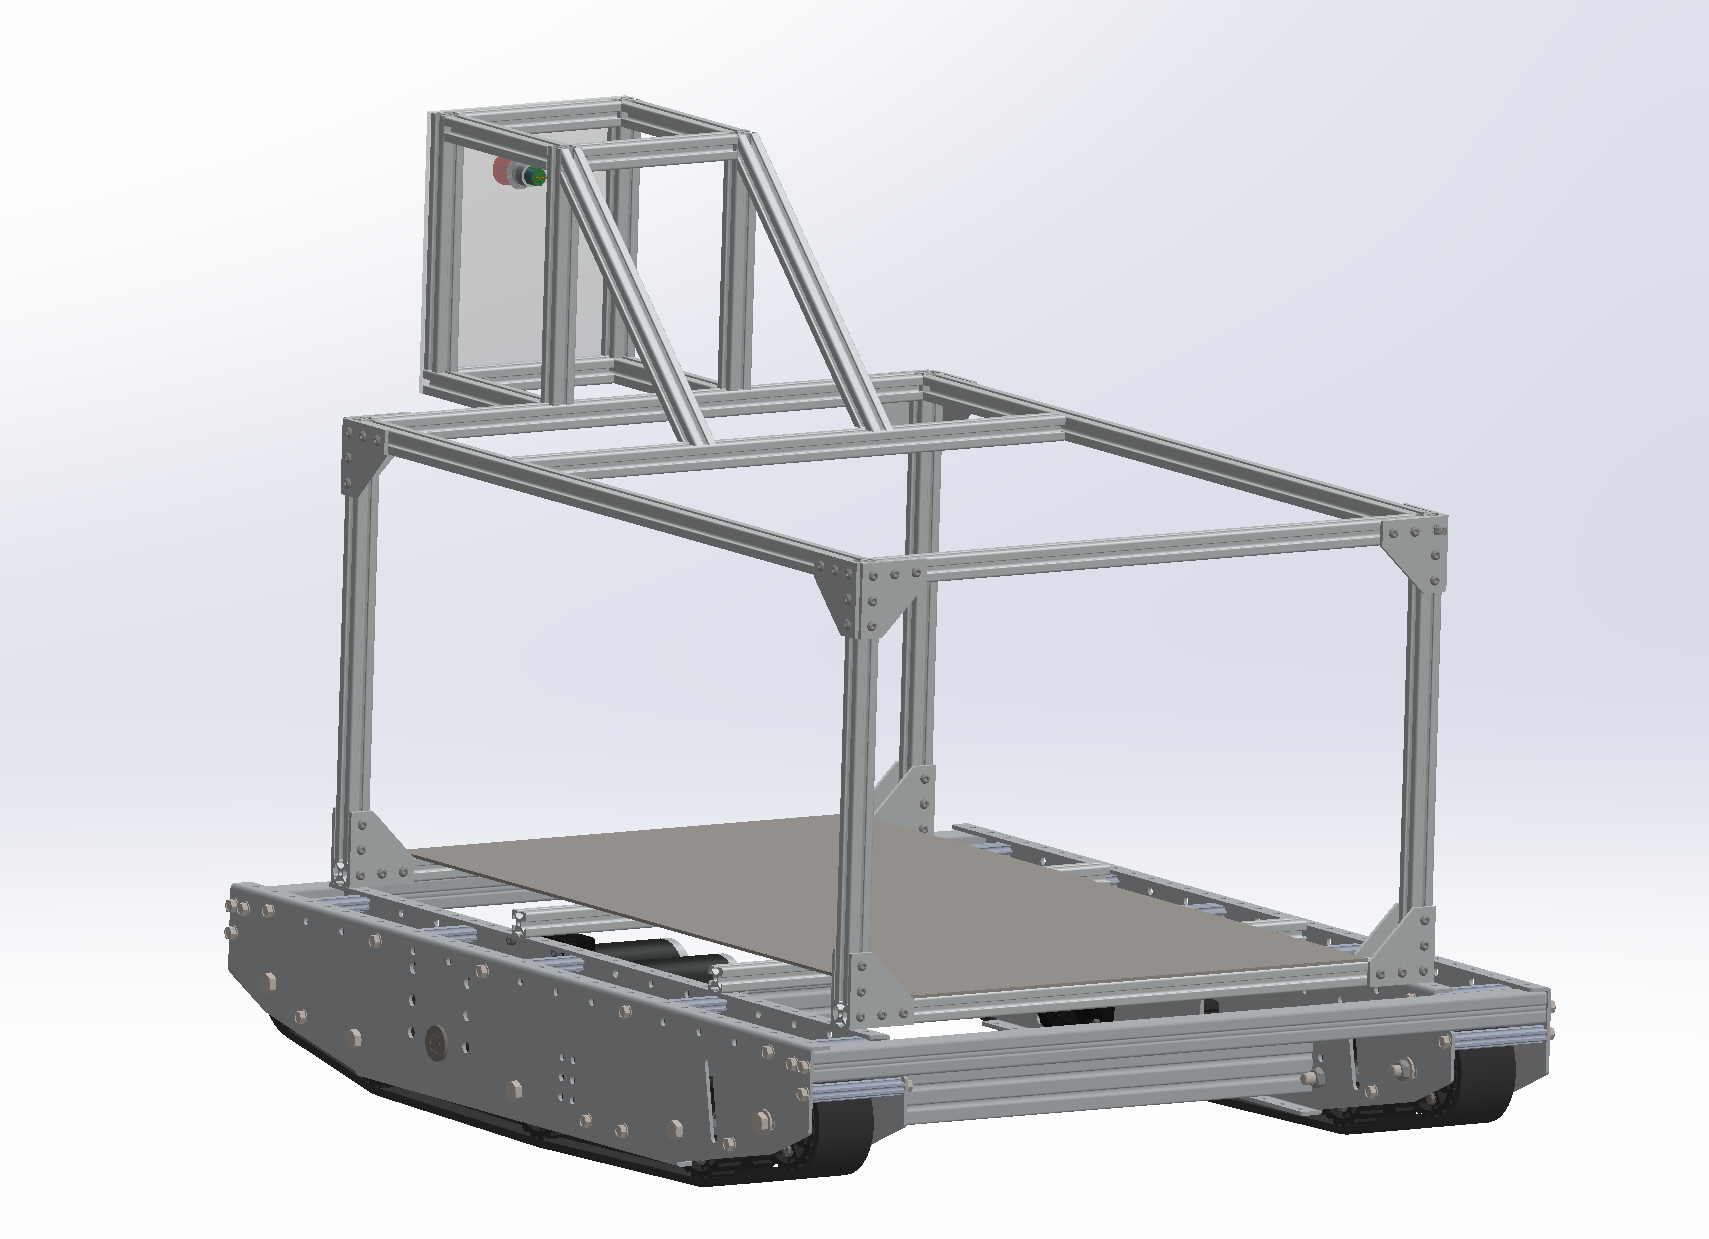
\includegraphics[width=0.45\textwidth]{figures/mech_image1.png}
    \hfill
    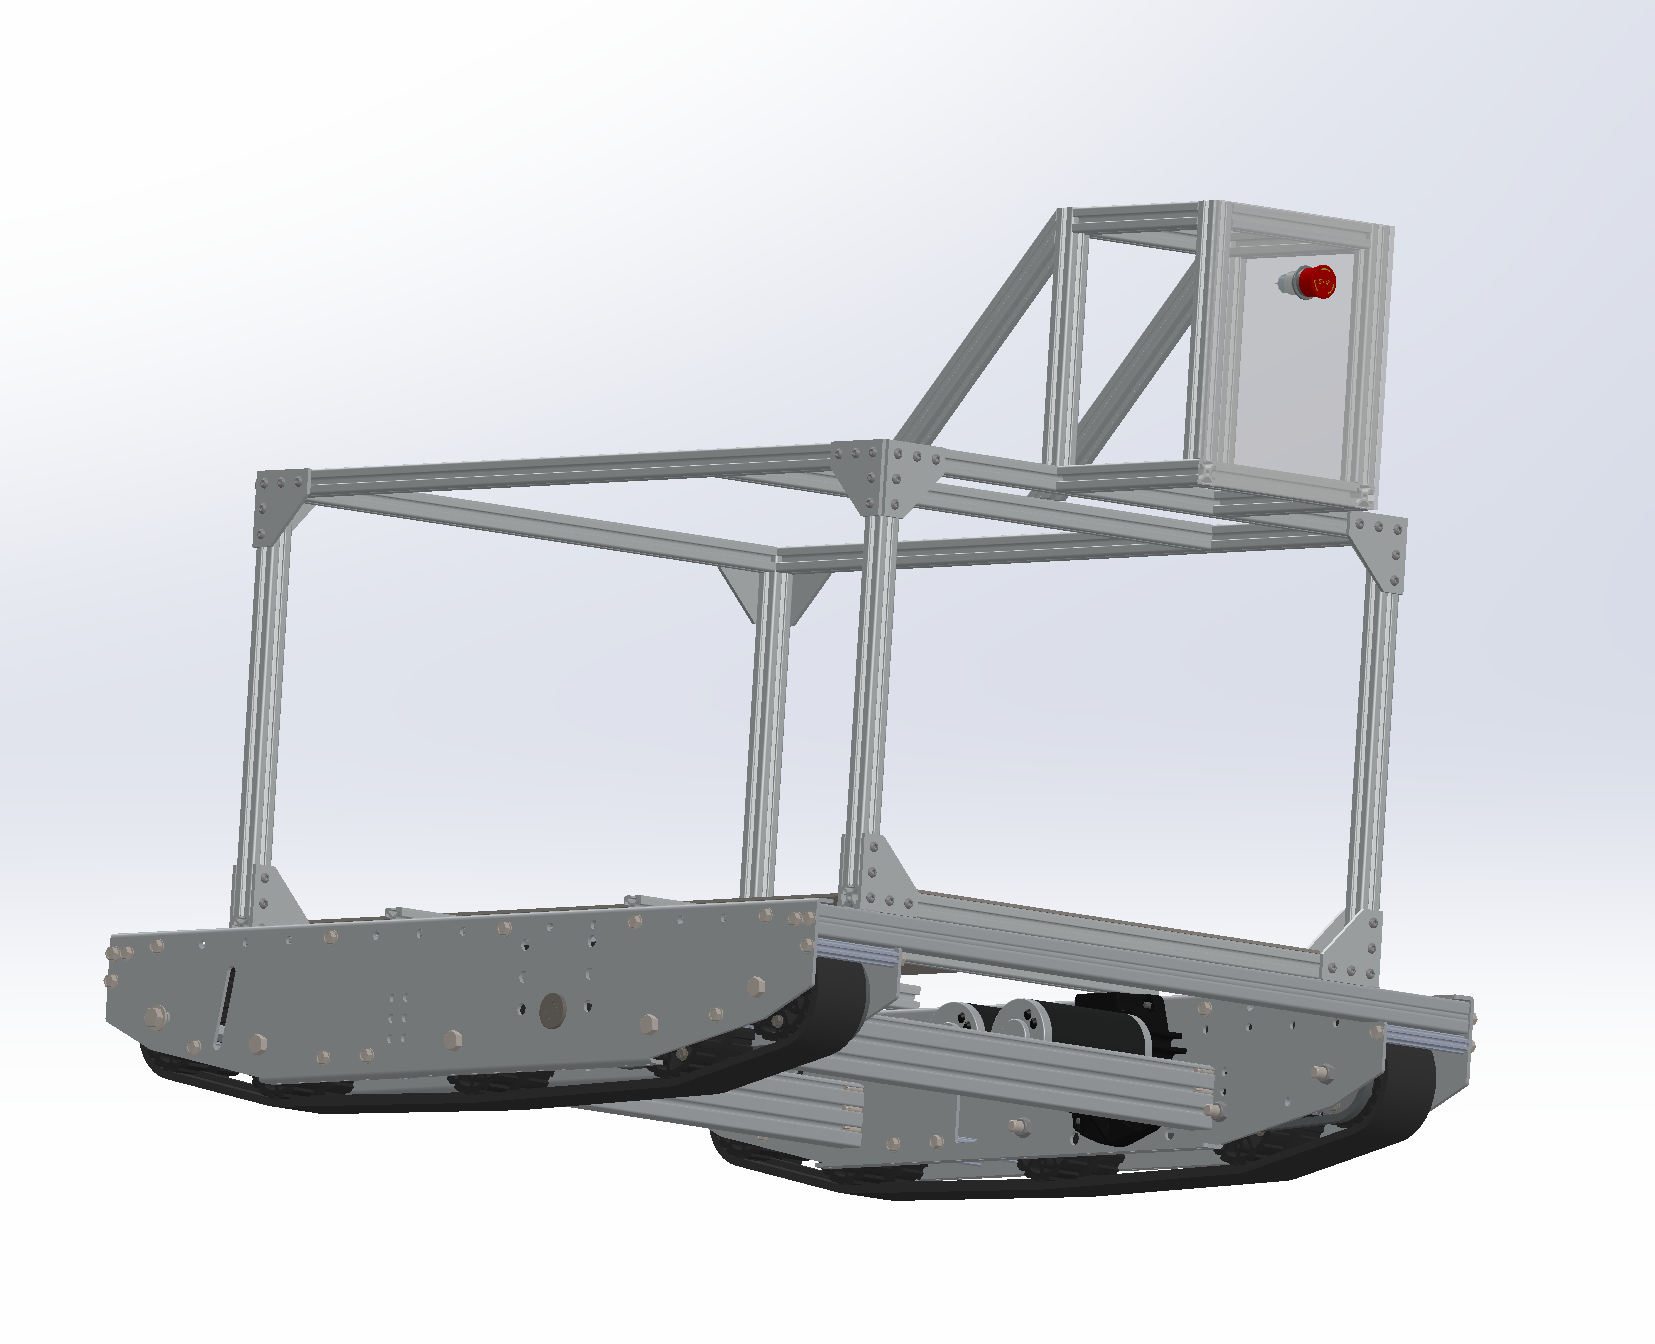
\includegraphics[width=0.45\textwidth]{figures/mech_image2.png}
    \caption{CAD renders of \textit{ROBOT NAME}: front view (left) and rear view (right).}
    \label{fig:mech_overview}
\end{figure}

\subsection{Drivetrain}

\textit{ROBOT NAME} utilizes a tracked differential drive system powered by two REV NEO brushless motors, each controlled by a REV SparkMAX motor controller. This configuration was chosen for both its mechanical and computational simplicity, as well as traction performance in outdoor environments.

The fixed belt-tracked system allows for skid-steer operation where each motor drives one side of the track independently. Straight motion is achieved when both motors rotate at the same speed in the same direction, while turning is accomplished by varying the relative speeds of each motor:

\begin{itemize}[nosep]
    \item \textbf{Pivot Turn} --- One track moves forward while the other stays still; the robot pivots around the stationary track.
    \item \textbf{In-Place Rotation (Spin)} --- The tracks rotate in opposite directions at the same speed ($v_L = -v_R$); the robot rotates around its center point.
    \item \textbf{Gradual Curve} --- One track rotates faster than the other ($v_L > v_R$ to turn right).
\end{itemize}

This approach eliminates the need for four independent motors or steering mechanisms, reducing system complexity in both mechanical design and control software. Using the track belts instead of regular wheels, the weight of \textit{ROBOT NAME} is spread over a larger area, increasing traction and stability across uneven terrain and obstacles encountered on the course.

\begin{table}[H]
\centering
\caption{Drivetrain specifications.}
\begin{tabularx}{\textwidth}{Xr}
\toprule
\textbf{Parameter} & \textbf{Value} \\
\midrule
Drive type           & Tracked differential (skid-steer) \\
Drive platform       & AndyMark Raptor Track Drive \\
Motors               & 2$\times$ REV NEO brushless \\
Motor controllers    & 2$\times$ REV SparkMAX \\
Gear ratio           & TODO \\
Designed top speed   & TODO \\
Track width          & TODO \\
\bottomrule
\end{tabularx}
\end{table}

\subsection{Frame and Sensor Mast}

The structural frame was constructed using 80/20\textsuperscript{\textregistered} 20-Series T-slot aluminum extrusions (80/20 Inc., USA). These extrusions allow for a modular and reconfigurable design that can be adapted for future competitions. To improve safety during assembly and operation, T-slot nuts were utilized within the extrusion channels, eliminating exposed threaded ends and reducing the risk of sharp edges. Attached to the base chassis is a 1/8\,in thick diamond plate steel base (21.5\,in $\times$ 30\,in), offering a rigid and large mounting surface for heavy components.

Weight distribution was a prioritized design consideration. The battery pack was mounted toward the rear of the chassis to act as a counterbalance to the 20\,lb payload, which was positioned toward the front of the vehicle on a 3D-printed mount. Electronics were centrally located and mounted on 3D-printed brackets attached to a carbon fiber plate, preventing direct contact with the steel base and protecting sensors and components from electrical interference.

A sensor mast is mounted at the center/front of the robot to elevate the camera(s) and GPS antenna. Maximizing the height of the cameras provides a wider field of view and allows the image to be projected onto a 2D plane with minimal distortion.

\subsection{Weatherproofing}

\textit{ROBOT NAME} utilizes acrylic panel walls integrated into the T-slot frame for protection from rain and sun. The acrylic sheets are cut-to-fit inside the T-slot extrusion grooves, with weatherstripping gaskets filling the gaps to ensure a secure fit that remains in place even with vibration during operation. The top panel is angled for water runoff and includes a sliding door for maintenance, wiring, and payload handling. All cable pass-throughs are sealed to prevent water ingress.

\subsection{Constraints}

To satisfy the competition size requirements, \textit{ROBOT NAME} was extended through the addition of an 8$\times$6\,in rear-mounted enclosure for the mechanical E-stop button, extending the length of the vehicle over the minimum 3\,ft required. This structure was mounted at 2\,ft from the ground, and the E-stop button was centrally positioned for easy access.

\newpage

% =============================================================================
% SECTION 5
% =============================================================================
\section{Electronic and Power Design}

\begin{figure}[H]
    \centering
    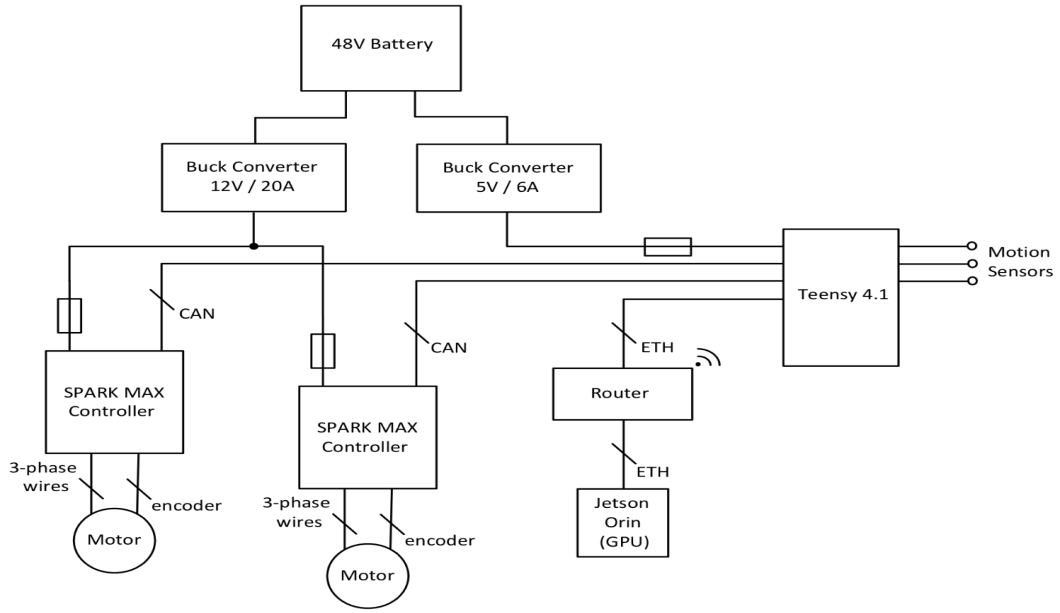
\includegraphics[width=0.95\textwidth]{figures/electrical_p1_img1.png}
    \caption{Electronic and power architecture of \textit{ROBOT NAME}.}
    \label{fig:elec_arch}
\end{figure}

\subsection{Overview}

The electronic system of \textit{ROBOT NAME} is designed for modularity and repairability. The architecture features the following key components:

\begin{itemize}[nosep]
    \item \textbf{NVIDIA Jetson Orin} --- Main onboard GPU computer for vision processing and object detection
    \item \textbf{Teensy 4.1} --- CAN bridge handling motor control and encoder feedback
    \item \textbf{CAN transceiver} --- SN65HVD230 converting logic-level to differential CAN
    \item \textbf{2$\times$ REV SparkMAX} --- Brushless motor controllers with built-in PID
    \item \textbf{Router} --- Central network hub connecting Jetson Orin and Teensy 4.1 via Ethernet, with Wi-Fi to remote laptop
    \item \textbf{E-stop system} --- Hardware relay controlled by physical + wireless + software interlocks
    \item \textbf{Safety lights} --- TODO: RGB LED strip / indicator lights
\end{itemize}

\subsection{Power Distribution}

The power system consists of a 48\,V battery wired to two separate buck converters. The first buck converter brings the voltage down to 12\,V with a maximum output of 20\,A, which provides sufficient current to the 12\,V motors via the SparkMAX controllers. The second buck converter brings the voltage down to 5\,V with a maximum output of 6\,A, which is used to power the Teensy 4.1 microcontroller. Both buck converters run through multiple fuses before reaching their respective devices, providing overcurrent protection throughout the power distribution system.

\begin{figure}[H]
    \centering
    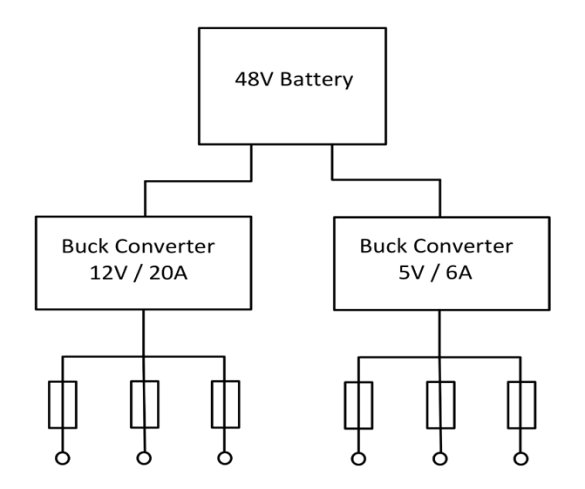
\includegraphics[width=0.5\textwidth]{figures/electrical_p1_img2.png}
    \caption{Power distribution topology: 48\,V battery to dual buck converters with fused outputs.}
    \label{fig:power_dist}
\end{figure}

\begin{table}[H]
\centering
\caption{Power budget.}
\begin{tabularx}{\textwidth}{Xrrr}
\toprule
\textbf{Component} & \textbf{Voltage (V)} & \textbf{Peak Current (A)} & \textbf{Avg Current (A)} \\
\midrule
Jetson Orin         & 5--20 (via buck) & TODO & TODO \\
Teensy 4.1          & 5 (via 5\,V/6\,A buck) & 0.1 & 0.05 \\
SparkMAX + motors   & 12 (via 12\,V/20\,A buck) & TODO & TODO \\
Sensors / cameras   & TODO & TODO & TODO \\
Safety lights       & TODO & TODO & TODO \\
\midrule
\textbf{Total}      & --- & TODO & TODO \\
\bottomrule
\end{tabularx}
\end{table}

\subsection{Computer Network}

The computer network is centered around a router that connects both the NVIDIA Jetson Orin and the Teensy 4.1 microcontroller via Ethernet. The Jetson Orin is used for computationally intensive tasks such as vision processing and object detection, while the Teensy 4.1 handles system data including motor control and sensor feedback over CAN bus. The router also transmits system data to a remote laptop via Wi-Fi, enabling real-time monitoring and debugging during operation.

\begin{figure}[H]
    \centering
    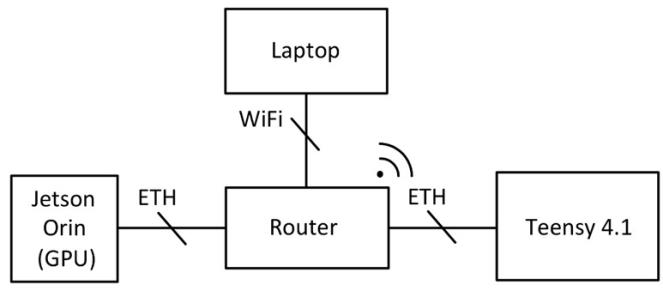
\includegraphics[width=0.6\textwidth]{figures/electrical_p2_img1.jpeg}
    \caption{Computer network topology.}
    \label{fig:network}
\end{figure}

\subsection{Motor Control}

\textit{ROBOT NAME} controls its two drive motors by commanding the SparkMAX controllers over a dedicated CAN bus. The Teensy 4.1 serves as the CAN bridge, translating high-level commands from the main computer (received over Ethernet via the onboard router) into SparkMAX CAN frames. Using the data received from the SparkMAX controllers, the system implements PID control to maintain correct speeds and position.

The SparkMAX controllers use REV Robotics' proprietary CAN protocol with 29-bit extended identifiers. The CAN ID is structured as follows:

\begin{table}[H]
\centering
\caption{SparkMAX CAN ID bit-field layout (29-bit extended).}
\begin{tabularx}{\textwidth}{Xccl}
\toprule
\textbf{Field} & \textbf{Bits} & \textbf{Width} & \textbf{Value} \\
\midrule
Device Type    & 28:24 & 5 bits & 2 (Motor Controller) \\
Manufacturer   & 23:16 & 8 bits & 5 (REV Robotics) \\
API Class      & 15:10 & 6 bits & Varies by command \\
API Index      & 9:6   & 4 bits & Varies by command \\
Device ID      & 5:0   & 6 bits & 1--62 (unique per controller) \\
\bottomrule
\end{tabularx}
\end{table}

Key API commands used:

\begin{itemize}[nosep]
    \item \textbf{Non-RIO Heartbeat} (Class 11, Index 2) --- Sent every 20\,ms to keep controllers enabled
    \item \textbf{Percent Output} (Class 0, Index 2) --- Motor duty cycle from $-1.0$ to $+1.0$
    \item \textbf{Velocity Setpoint} (Class 1, Index 2) --- Target RPM using SparkMAX internal PID
    \item \textbf{Encoder Feedback} (Class 6, Index 2) --- Periodic drive encoder position reports
\end{itemize}

All floating-point values are encoded as IEEE 754 single-precision floats in little-endian byte order. By offloading the PID control loop onto the SparkMAX controllers, we simplify the firmware and reduce end-to-end latency.

\subsection{Safety Lights}

Safety lights on the vehicle indicate the autonomous state as required by IGVC rules.

\begin{table}[H]
\centering
\caption{Safety light color mapping.}
\begin{tabularx}{\textwidth}{lX}
\toprule
\textbf{Light Color} & \textbf{Meaning} \\
\midrule
White   & Standard operation \\
Yellow  & Waypoint following activated \\
Green   & Waypoint reached \\
Red     & Unable to move forward / error \\
\bottomrule
\end{tabularx}
\end{table}

\subsection{Emergency Stop and Safety}

Safety is a top priority for the vehicle and is at the core of our electrical design. The emergency stop circuit features three interlocks that must all be disengaged for the motors to receive power:

\begin{enumerate}[nosep]
    \item \textbf{On-vehicle button} --- Physical red mushroom-head e-stop button.
    \item \textbf{Remote button} --- Wireless e-stop with $>$100\,ft range, as required by IGVC rules.
    \item \textbf{Software interlock} --- Software-controlled relay that is only enabled when all nodes report healthy status.
\end{enumerate}

Motor power is gated by a solid-state relay controlled directly by the e-stop line. If any interlock is triggered, power to the motor controllers is immediately cut regardless of software state.

\newpage

% =============================================================================
% SECTION 6
% =============================================================================
\section{Software Systems}

\subsection{Overview}

Our software uses the \textbf{Robot Operating System (ROS 2)}, a robotics middleware that is widely used in both academia and industry. It is based on a publisher-subscriber model, with individual processes called nodes sending messages to each other. This allows for much of the software work to be developed in parallel in separate packages.

% \begin{figure}[H]
%     \centering
%     \includegraphics[width=0.9\textwidth]{figures/vision_pipeline.png}
%     \caption{Vision processing pipeline.}
%     \label{fig:vision}
% \end{figure}

\subsection{Image Transformation}

\textit{ROBOT NAME} uses a classical computer vision approach to transform camera image(s) into an obstacle map that the vehicle can use to navigate.

The images are processed through the following pipeline:

\begin{enumerate}[nosep]
    \item \textbf{Camera calibration} --- Correct lens distortion using a calibration matrix.
    \item \textbf{Perspective transform} --- Project the camera image onto a top-down 2D plane.
    \item \textbf{Color filtering} --- Apply HSV thresholding to detect lane lines and obstacles.
    \item \textbf{Obstacle map generation} --- Combine filtered images into a unified obstacle map.
\end{enumerate}

TODO: Describe any auto-calibration or adaptation to lighting conditions.

\subsection{Navigation}

TODO: Describe your path planning and navigation algorithm.

The navigation system receives the obstacle map from the perception subsystem and the current position from the localization subsystem. It computes motor commands that guide the vehicle toward the next GPS waypoint while avoiding detected obstacles.

\subsection{Localization}

Autonomous localization is required for qualifying for and completing the IGVC AutoNav challenge. Waypoint navigation is only possible with accurate and precise location data.

\textit{ROBOT NAME} uses a particle filter / extended Kalman filter that combines:
\begin{itemize}[nosep]
    \item \textbf{Track odometry} --- Encoder feedback from the SparkMAX motor controllers, transmitted through the Teensy 4.1 over CAN bus.
    \item \textbf{GPS data} --- TODO: GPS module name and accuracy specifications.
    \item \textbf{IMU data} --- TODO: IMU name providing heading and angular velocity (motion sensors connected to Teensy 4.1).
\end{itemize}

This fused location data is consumed by the path planner as the robot's current position and is used to determine waypoint arrival and distance from the start of the course.

\subsection{Drive Control}

The Jetson Orin publishes desired linear and angular velocity commands. These are converted to individual left/right track speeds using the differential drive kinematic model:

\begin{align}
    v_L &= v - \frac{\omega \cdot d}{2} \\
    v_R &= v + \frac{\omega \cdot d}{2}
\end{align}

where $v$ is the desired linear velocity, $\omega$ is the desired angular velocity, and $d$ is the track width (distance between track centers).

The computed track speeds are sent to the Teensy 4.1 over Ethernet (via the onboard router), which translates them into SparkMAX CAN commands. Encoder feedback from both motors is read by the Teensy and sent back to the Jetson Orin for odometry computation.

\subsection{Configuration and GUI}

TODO: Describe any GUI, configuration system, or parameter tuning tools.

Configuration of tunable parameters is handled via a custom GUI / ROS parameter server running on the main computer. This allows the team to tune the robot on-the-fly without recompiling code.

\subsection{State Machine}

The robot operates using a state machine that manages transitions between the following system states:

\begin{itemize}[nosep]
    \item \textbf{Disabled} --- Motors off, all subsystems idle.
    \item \textbf{Manual} --- Operator control via gamepad/controller for testing.
    \item \textbf{Autonomous} --- Full autonomy, running perception + navigation + localization.
    \item \textbf{Emergency Stop} --- Immediate motor cutoff, requires manual reset.
\end{itemize}

Each software node also maintains its own local state (off, warming, ready, operating, error) to ensure all subsystems are healthy before autonomous operation begins.

\subsection{Logging}

TODO: Describe your data logging strategy for post-run analysis.

After every run, a comprehensive log file is created containing sensor readings (camera feeds, GPS, IMU, encoder feedback), diagnostic metrics, navigation targets, and debug information.

\newpage

% =============================================================================
% SECTION 7
% =============================================================================
\section{Cyber Security Analysis}

\subsection{NIST RMF Process}

Security vulnerabilities in self-driving vehicles pose significant risks. To effectively mitigate these threats, the team follows the NIST Risk Management Framework (RMF), which provides a structured process for identifying, assessing, and managing risks throughout the system's life cycle.

\subsection{Vehicle Threats}

\begin{table}[H]
\centering
\caption{Threat assessment matrix.}
\begin{tabularx}{\textwidth}{lXccc}
\toprule
\textbf{Subsystem} & \textbf{Threat Description} & \textbf{Confid.} & \textbf{Integrity} & \textbf{Avail.} \\
\midrule
GPS Waypoints    & GPS waypoint tampering could lead the vehicle to drive in unintended ways. & Low & High & High \\
\addlinespace
Remote E-stop    & Malicious interference could disable or trigger the e-stop. & Moderate & High & High \\
\addlinespace
Onboard Computer & Malware or unauthorized access could compromise system control. & High & High & High \\
\addlinespace
Odometry         & Sensor data tampering can result in incorrect state estimation. & Low & High & Moderate \\
\addlinespace
CAN Bus          & CAN frame injection could send unauthorized motor commands. & Moderate & High & High \\
\addlinespace
Git Repository   & Unauthorized access could inject malicious code. & High & High & Moderate \\
\bottomrule
\end{tabularx}
\end{table}

\subsection{Cyber Controls and Implementation}

\begin{table}[H]
\centering
\caption{Security controls.}
\begin{tabularx}{\textwidth}{lXX}
\toprule
\textbf{Subsystem} & \textbf{Control} & \textbf{Implementation} \\
\midrule
GPS Waypoints    & SI-4 System Monitoring & Display GPS waypoints to the user and validate using range checks. \\
\addlinespace
Remote E-stop    & AC-3 Access Enforcement & Authenticate and/or encrypt the e-stop radio channel. \\
\addlinespace
Onboard Computer & SC-28 Protection of Information at Rest & Use secure boot, enable SSH authentication, and disable passwords. \\
\addlinespace
Odometry         & SI-7 Information Integrity & Validate sensor input using range checks and sensor fusion. \\
\addlinespace
CAN Bus          & SC-8 Transmission Confidentiality & Monitor for anomalous CAN traffic; heartbeat watchdog timeout. \\
\addlinespace
Git Repository   & CM-5 Access Restrictions for Change & Enforce code access control with role-based permissions. \\
\bottomrule
\end{tabularx}
\end{table}

\newpage

% =============================================================================
% SECTION 8
% =============================================================================
\section{Vehicle Analysis}

\subsection{Lessons Learned}

TODO: Describe the key lessons your team learned during the design and build process.

\subsection{Failure Points and Resolutions}

\begin{table}[H]
\centering
\caption{Failure points and resolutions.}
\begin{tabularx}{\textwidth}{lXXX}
\toprule
\textbf{Category} & \textbf{Failure Point} & \textbf{Cause} & \textbf{Resolution} \\
\midrule
Mechanical  & Fasteners loosen & Vibrations from driving & Loctite and Nyloc nuts \\
\addlinespace
Electrical  & E-stop connection lost & Remote goes out of range & Heartbeat timeout stops robot \\
\addlinespace
Electrical  & CAN bus errors & Wiring / termination issues & Added proper 120\,$\Omega$ termination \\
\addlinespace
Software    & Obstacle misdetection & Changing weather / lighting & Auto HSV calibration at startup \\
\addlinespace
Software    & Sensor data loss & Cable disconnect / node crash & Watchdog monitors node health \\
\bottomrule
\end{tabularx}
\end{table}

\subsection{Safety, Reliability, and Durability}

\textit{ROBOT NAME} was designed from the ground up to be safe, reliable, and durable in all conditions. Through dozens of test runs in various scenarios---sensor loss, changing weather conditions, e-stop testing---the team has verified that the robot reliably activates all of its safety measures.

TODO: Describe specific reliability testing you performed.

\subsection{Performance Metrics}

\begin{table}[H]
\centering
\caption{Performance metrics.}
\begin{tabularx}{\textwidth}{Xlr}
\toprule
\textbf{Parameter} & \textbf{Requirement} & \textbf{Measured Value} \\
\midrule
Course Completion Time   & $<$5 minutes   & TODO \\
Obstacle Detection Range & $>$2 meters    & TODO \\
Obstacle Reaction Time   & $<$250 ms      & TODO \\
Remote E-stop Range      & $>$100 ft      & TODO \\
Navigation Accuracy      & $<$1 meter     & TODO \\
Battery Life             & $>$5 minutes   & TODO \\
Ramp Ascension           & Successful     & TODO \\
\bottomrule
\end{tabularx}
\end{table}

\subsection{Software Testing, Bug Tracking, and Version Control}

The software subteam utilizes Git and GitHub to store and version control the codebase. By utilizing branches for each new feature, those features can be isolated and independently tested before being merged into the main codebase.

TODO: Describe your CI/CD pipeline, testing framework, and bug tracking process.

\subsection{Simulation}

TODO: Describe any simulation environment you use (Gazebo, custom simulator, Unity, etc.).

% \begin{figure}[H]
%     \centering
%     \includegraphics[width=0.7\textwidth]{figures/simulation.png}
%     \caption{Simulation environment.}
%     \label{fig:sim}
% \end{figure}

\newpage

% =============================================================================
% SECTION 9
% =============================================================================
\section{Unique AutoNav and Self Drive Software}

\textit{ROBOT NAME} is competing in AutoNav only / is competing in both AutoNav and Self Drive.

AutoNav and Self Drive share many core features such as lane keeping and obstacle avoidance. However, Self Drive requires additional capabilities such as:

\begin{itemize}[nosep]
    \item Lane changing
    \item Stop sign detection and compliance
    \item Merging
    \item Parking
\end{itemize}

TODO: Describe any unique software features for each mode.

\newpage

% =============================================================================
% SECTION 10
% =============================================================================
\section{Performance Assessment}

As of submitting this report, \textit{ROBOT NAME} is on track for competition. Through extensive testing, the drivetrain, vision pipeline, and navigation systems have been validated.

TODO: Summarize overall readiness for competition. Be honest about what is complete and what remains.

\end{document}
